\documentclass[11pt,a4paper]{article}
% \renewcommand\normalsize{\fontsize{12}{18.0pt}\selectfont}
\usepackage[utf8]{inputenc}
\usepackage[T2A]{fontenc}
\usepackage[russian]{babel}
\usepackage{graphicx}
\usepackage{amsmath,amssymb,amsthm}
\usepackage{epsfig}
\usepackage{import}
\usepackage{wrapfig}
\usepackage{epigraph}
\usepackage{verbatim}
\usepackage{soul}
\usepackage[usenames]{color}
\usepackage{listings}
\usepackage{pdfpages}

\pagestyle{empty}

\hoffset=-15mm    %по горизонтали влево на \hoffset
\voffset=-37.5mm  %по вертикали вверх на \voffset
\textheight=275mm
\textwidth=155mm


\newcommand{\eps}{\varepsilon}
\renewcommand{\phi}{\varphi}
\newcommand{\Impl}{\ensuremath{\Rightarrow}}
\newcommand{\RRR}{\overline{\mathbb{R}}}
\newcommand{\RR}{\mathbb{R}}
\newcommand{\NN}{\mathbb{N}}
\newcommand{\QQ}{\mathbb{Q}}
\newcommand{\nl}{\newline}

\usepackage{ifthen}
\newcommand\ifnonempty[2]{\ifthenelse{\equal{#1}{}}{}{#2}}
% Команда \task для условий задач с одним необязательным аргументом
% \defin определения, \exerc упражнения \prop предложения \theor теорема
\newcounter{task}
\newcounter{defin}
\newcounter{prop}
\newcounter{thm}
\newcommand{\task}[1][]{\smallskip\par\hangafter=1\normalsize\textbf{Задача \refstepcounter{task}\thetask\ifnonempty{#1}{ (#1)}.}~}
\newcommand{\defin}[1][]{\smallskip\par\hangafter=1\normalsize\textbf{Определение \refstepcounter{defin}\thedefin\ifnonempty{#1}{ (#1)}.}~}
\newcommand{\exerc}[1][]{\smallskip\par\hangafter=1\normalsize\textbf{Упражнение \refstepcounter{task}\thetask\ifnonempty{#1}{ (#1)}.}~}
\newcommand{\prop}[1][]{\smallskip\par\hangafter=1\normalsize\textbf{Предложение \refstepcounter{prop}\theprop\ifnonempty{#1}{ (#1)}.}~}
\newcommand{\thm}[1][]{\smallskip\par\hangafter=1\normalsize\textbf{Теорема \refstepcounter{thm}\thethm\ifnonempty{#1}{ (#1)}.}~}

\setcounter{thm}{2}

\begin{document}
\begin{center}
\Huge {
\noindent
\textbf{Задача о минимальной надстроке}
}
\end{center}
\begin{center}
Жуков Владислав 499
\end{center}
\defin
Пусть задано множество строк $A = \alpha_1, \alpha_2, ..., \alpha_n$ над конечным алфавитом. Требуется найти такую строку $\omega$, что
все строки из множества $A$ являются подстроками $\omega$ и длина $\omega$ минимальна. Назовем эту задачу "задачей о надстроке" или SSP.
\defin $IN(v), OUT(v)$ - обозначают количество входящих и выходящих ребер соответственно из вершины v.
\defin (Задача об ограниченном направленном Гамильтоновом пути)
\\
\textit{Задача напревленного Гамильтонова пути:}
\par Дан ориентированный граф $G$, есть ли в нем путь проходящий по всем вершинам ровно по одному разу.  Про эту задачу известно, что он NP-полная.
\\
\textit{Задача ограниченного направленного Гамильтонова пути:}
\par Это задача направленного Гамильтонова пути сго следующими ограничениями:
\\Есть назначенная стартовая вершина $s$ и конечная вершина $t$, такие, что $IN(s) = OUT(t) = 0$
\\Все вершины кроме конечной вершины $t$, имеют исходящую степень большую 1.
\defin
$overlap(s_1, s_2)$ Это длина наибольшего x, такого что $s_1 = ax$ и $s_2 = xb$ для некоторых строк $a$ и $b$. Проще говоря, это длина максимально возможного перекрытия двух строк.

\thm
SSP с бесконечным алфавитом является  NP-полной.
%Более того, это задача NP-полна даже если для любого $H \ge 3$, при ограничении на то, что все строки примитивные длины H
\par
\textit{Доказательство:}
% Для начала докажем для неприметивных строк длины 3, а после покажем как изменить конструкцию, чтобы сделать все строки примитивными длины H, для $H \ge 3$.
Пусть $G = (V, E)$ это граф из задачи ограниченного напревленного Гамильтонова пути, где $V$ это множество целых чисел от 1 до n(1 это начальная вершина и n это конечная вершина) и $|E| = m$.
Мы построим строки для $G$ над алфавитом $\Sigma = V \cup B \cup S$, где $B = \{\overline{v}| v \in V - \{n\} \}$ множество "запрещенных" символов", а S - множество специальных символов.
Запрещенные символы являются "локальными" для каждой вершины, тогда как специальные являются глобальными символами для всего графа $G$.
Для каждой вершины $v \in V - \{v\}$ мы сопоставим множество $A_v$ содержащее $2OUT(v)$ строк. Пусть $R_v = \{\omega_0, ..., \omega_{OUT(v) - 1}\}$ это множество вершин соединенных с $v$.
Тогда, $A_v = \{\overline{v}\omega_i\overline{v}|\omega_i \in R_v\} \cup \{\omega_i \overline{v}\omega_{i \oplus 1}| \omega_i \in R_v\}$, где $\oplus$ обозначает сложение по модулю $OUT(v)$.
\par
Для каждой вершины $v \in V - \{1, n\}$ создаем множество $C_v$ из одного элемента, содержащее строку $v \# \overline{v}$ называемую соединителем или коннектором.
Введем множество, которое содержит терминальные строки $T = \{\%\#\overline{1}, n\#\$\}$. Пусть S это объединение $A_j, 1 \le j < n$; $C_j, 1 \le i < n$ и T.
Утверждается, что G имеет направленный Гамильтонов путь в том и только в том случае, если S имеет надстроку длины $2m + 3n$.
\par
Предположим, что в $G$ есть направленный Гамильтонов путь. Пусть $v, \omega_i$ ребро из этого пути. Для начала построим надстроку длины $2OUT(v) + 2$ для $A_v$ вида
$\overline{v}\omega_i\overline{v}\omega_{i \oplus 1}\overline{v}...\overline{v}\omega_i$, называемую $\omega_i$-стандартной надстрокой для $A_v$.
Эта надстрока сформирована "схлапыванием" перекрытий строк $A_v$ в порядке
\begin{center}
$\overline{v}\omega_i\overline{v}, \omega_i\overline{v}\omega_{i \oplus 1}, \overline{v}\omega_{i \oplus1}\overline{v}, ...,
\overline{v}\omega_{i \oplus OUT(v)}\overline{v}, \omega_{i \oplus OUT(v)}\overline{v}\omega_i$
\end{center}
, где каждая последующая пара имеет перекрытие длины 2.
 Отметим, что множество $\omega_i$-стандартных надстрок для $A_v$ переходят друг в друга в соответствии с циклическими перестановками целых чисел от $0$ до $OUT(v) - 1$
Пусть $u_1, u_2, ..., u_n$ обозначает направленный Гамильтонов путь где $u_1 = 1, u_n = n$ и обозначим стандартную $u_j$ надстроку для $A_{u_i}$ как $STD(\overline{u_i}, u_j)$.
Мы можем построить надстроку для для S как схлапывание стандартных надстрок и строк из $S$ в конкретном порядке:
\begin{center}
$\%\#\overline{1}, STD(\overline{1}, u_2), u_2 \# \overline{u_2}, STD(\overline{u_2}, u_3), u_3\#\overline{u_3}, ...
\overline{u_{n - 1}}\#\overline{u_{n - 1}}, STD(\overline{n_{n - 1}}, n), n\#\$$
\end{center}
Надстрока имеет длину $\sum\limits_{i = 1}^{n - 1} (2OUT(i) + 2) + (n - 2) + 4 = 2m + 3n$.
\par
Чтобы доказать обратное утверждение, мы покажем, что $2m + 3n$ это нижняя граница размера надстроки $S$ и затем покажем, что эта нижняя граница может быть достигнута только в случае если надстрока
кодирует Гамильтонов путь. Всего мы имеем $2m + n$ строк, в сумме их длина $3(2m + n)$. Наибольшее "сжатие" дает порядок, в котором каждая строка кроме первой имеет перекрытие длины 2 с обеих сторон.
Этот порядок должен дать надстроку длины $3(2m + n) - 2(2m + n - 1) = 2m + n + 2$. Однако, n - 2 коннектора могут иметь перекрытие только длины 1 с обеих сторон,
т.к. ни одна строка не начинается и не заканчивается с символа $\#$.
К тому же терминальные строки могут перекрываться максимум на 1 символ только с одной строны. Соблюдая эти условия, мы имеем нижнюю границу на длину надстроки в
$(2m + n + 2) + 2(n - 2) + 2 = 2m + 3n$ для S. Отметим, что она начинается с $\%\#\overline{1}$ и заканчивается $n\#\$$.
Рассмотрим два вхождения $\#$ в такую надстроку. Обозначим за $x$ то, что находится между этими двумя знаками $\#$. Первый символ из $x$ должен быть запрещенным, а
последний не запрещенным, поскольку они являются подстрокой соединителя. Если в $x$ нет соеденителей, то тогда все подстроки кроме первой и последней должны иметь перекрытие 2 с обеих сторон.
Первая строка должна быть $\overline{v}u_j\overline{v}$, следующая $u_j\overline{v}u_{j \oplus 1}$ и так далее. Более того, все строки в $A_v$ кроме двух последних должны иметь перекрытие длины 2
с обеих сторон, так каждая последующая строка должна быть "добита" уникальной строкой, которая перекрывается с ней на 2 символа. Таким образом все строки в $A_v$ должны появляться в
конкретном порядке, и если $x$ содержит одну строку из $A_v$, то он обязан содержать их все. Таким образом, $x$ - это стандартная надстрока для $A_v$
Применяя рассуждения выше ко всем вхождениям пар $\#$ мы получаем $n - 1$ различную стандартную строку. Мы можем восстановить Гамильтонов путь смотря на символы следующие за каждым вхождением $\#$,
причем запрещенные и не запрещенные символы каждого соединителя отвечают одной и той же верщине в $G$. Отметим, что в силу расположения $\%\#\overline{1}$ и $b\#\$$, мы получаем путь из $1$ в $n$
\\
\begin{center}
\Large
\textbf{4 приближенный алгоритм}
\normalsize
\end{center}
\par
Построим граф $G = (V, E)$, где $V = 1..n, E = \{(i, j, overlap(s_i, s_j))| i, j = 1..n, i \ne j\}$ - последнее множество,
это множество троек (начальная вершина, конечная вершина, вес). Затем для данного графа $G$ найдем покрытие циклами минимального суммарного веса.
Это и будет 4-приближенный алгоритм для задачи.
\par
\textit{Вычислим жадное назначение для данного графа $G$}
\\
Будем хранить его в массиве из n чисел, обозначим его за $A$.
\\
объявим все ребра незачеркнутыми\\
повторять пока остаются незачеркнутые ребра.\\
1)Выберем ребро (i, j) максимального веса среди незачеркнутых\\
2)Зачеркнем все рабра выходящие из i и входящие в j\\
3)A[i] = j
\par
\textit{Наконец найдем покрытие минимального суммарного веса}\\
0)Повторям пока есть непосещенные вершины.
\\
1) Возьмем вершину непосещенную вершину $i$. Отметим как посещенную. Положим $s = i$\\
2)while True:\\
Далее если $A[i]$ совпадает с $s$, то добавим цикл в результат, закончить цикл, перейти к пункту $(0)$\\
иначе $i = A[i]$
\begin{center}
\Large
\textbf{Запуски, проверка 2-приближенности жадного алгоритма для маленьких строк}
\normalsize
\end{center}
Далее приведен Ipython notebook. К сожалению nbpdfconverter не поддерживает кириллицу, поэтому пояснения приведены на английском.

\setboolean{@twoside}{false}
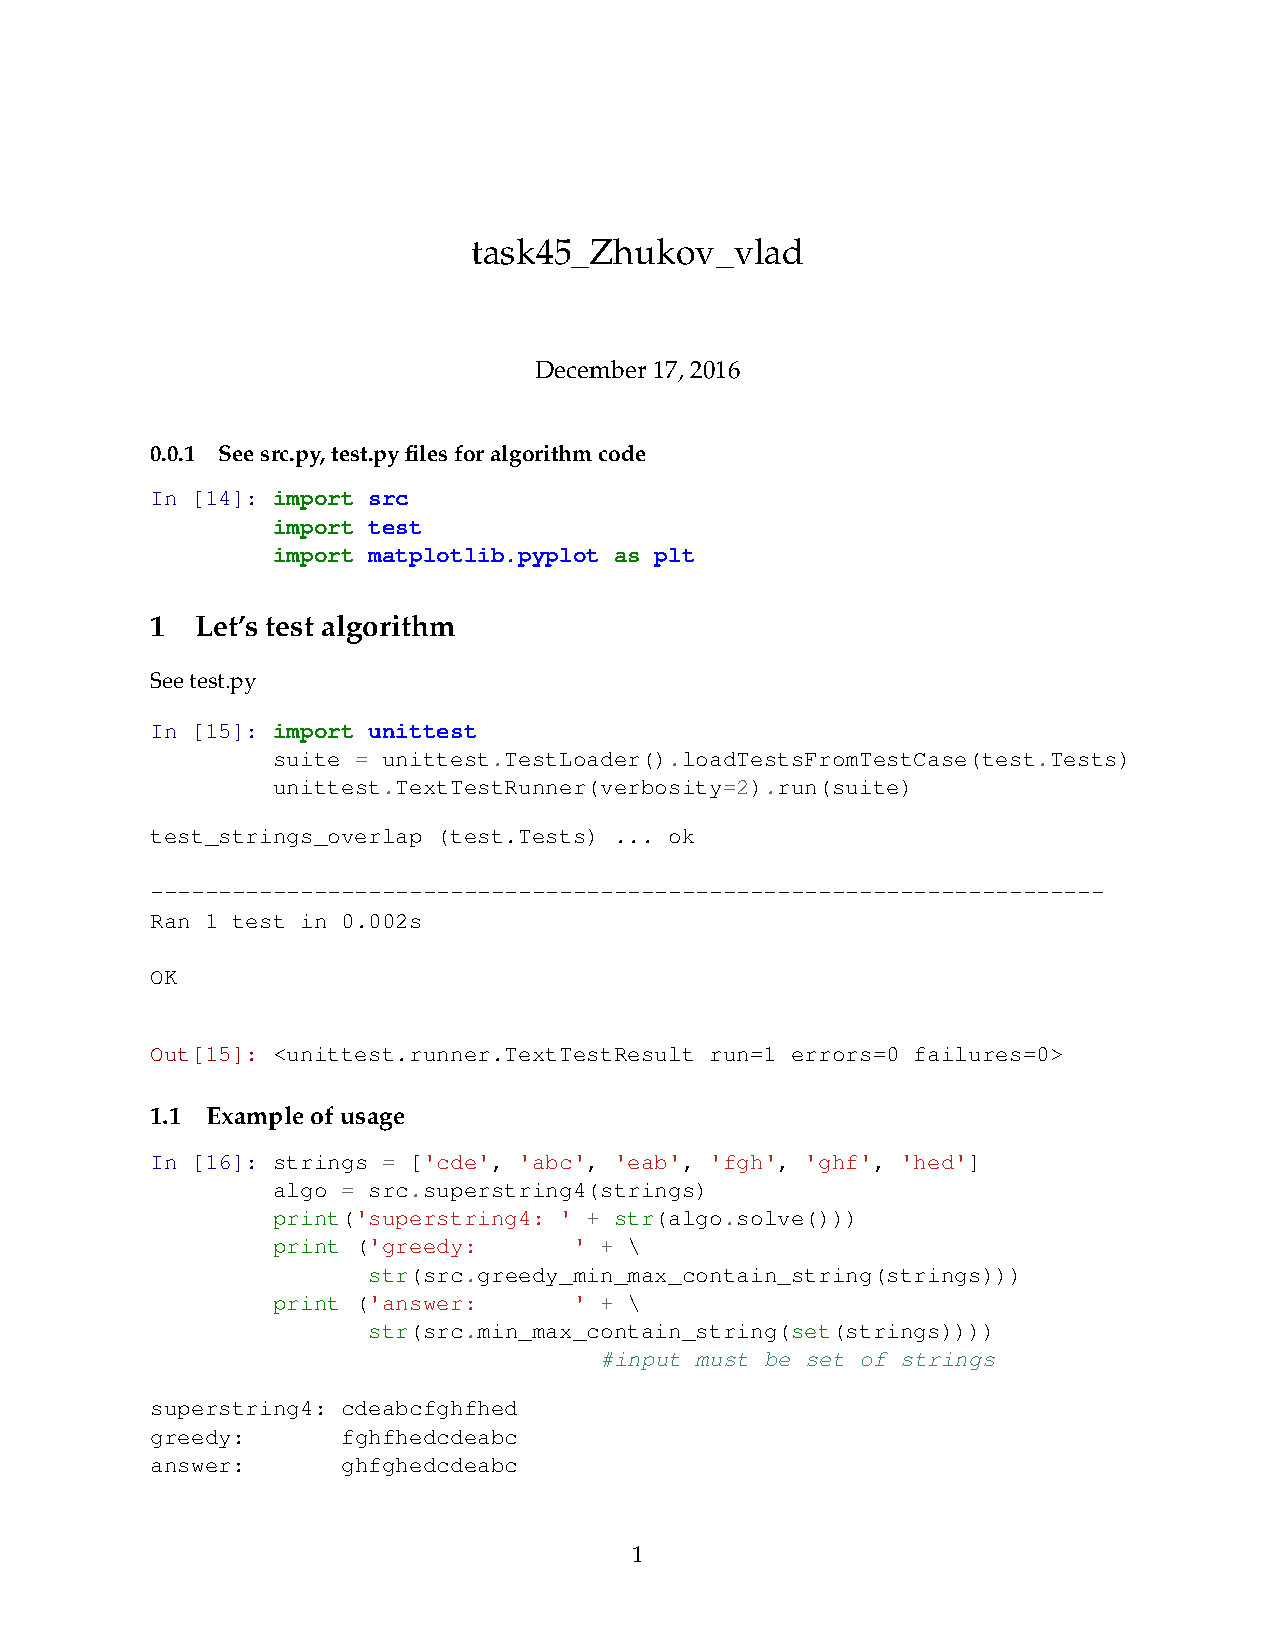
\includepdf[pages=-, offset=15 -75]{notebook.pdf}
\begin{center}
\Large
\textbf{Имплементация алгоритмов. src.py}
\normalsize
\end{center}
\par
\lstset{
  caption=Descriptive Caption Text,
  basicstyle=\footnotesize, frame=tb,
  xleftmargin=-.0\textwidth, xrightmargin=.2\textwidth
}
\lstinputlisting[language=Python]{src.py}
\begin{center}
\Large
\textbf{test.py}
\normalsize
\end{center}
\lstinputlisting[language=Python]{test.py}

\begin{thebibliography}{9}
\bibitem{lamport94}
 J Gallant, D Maier, J Astorer
  \emph{ On finding minimal length superstrings},
  Journal of Computer and System Sciences, 1980 - Elsevier
\bibitem{lamport94}
  Jonathan S. Turner
  \emph{ APPROXIMATION ALGORITHMS FOR THE SHORTEST COMMON SUPERSTRING PROBLEM},
  Computer Science Department Washington University, St. Louis
\bibitem{lamport94}
Marcin Mucha
  \emph{A Tutorial on Shortest Superstring Approximation}
  December 17, 2007
\end{thebibliography}
\end{document}
